\subsection{Метод за следене използвайки ултразвук за увеличена реалност}

В документ \cite{vr} се описва система изградена от 4 получателя, които са позиционирани в ъглите на региона. Описани са 3 равнини [фиг. \ref{fig:planes}], които се използват за изчислението на координатите на точките. Това е еквивалентно на линеризиране на уравненията, за което в \cite{murphy} е споменато като метод, който не дава задоволителни резултати в реални условия.  Изчисленията на координатите се извършват с помощта на  Питагоровата теорема. За целта се използват  следните уравнения. \\

\centerline{
    \begin{equation}
        k=i+2
    \end{equation}
}

\centerline{
    \begin{equation} \label{22eq}
        \begin{bmatrix}
                $(x_i - x)^2 + y^2 = d_i_2$\\
                $(x_k - x)^2 + y^2 = d^2_k$
        \end{bmatrix}
    \end{equation}
}

\begin{figure}
    \centering
    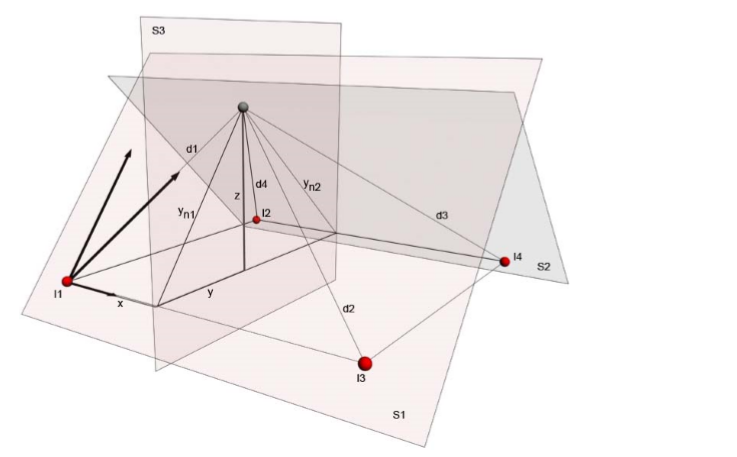
\includegraphics{planes}
    \caption{Равнините използвани за пресмятането на координатите}
    \label{fig:planes}
\end{figure}